\label{sec:ed}
The TU/e \acrfull{ed} is a \acrfull{ros} based 3D geometric, object-based world representation system for robots. In itself ED is a database system that structures multi-modal sensor information and represents this in an object-based world representation that can be utilized for robot localisation, navigation, manipulation and interaction functions. Figure \ref{fig:ed} shows a schematic overview of ED.

ED has been used on our robots AMIGO and SERGIO in the OPL for many years and is now also used on the Toyota HSR in DSPL. In previous years, developments have been focussed on making ED platform independent. As a result ED has been used on the PR2 system, Turtlebot and Dr. Robot systems (X80). Also multiple other @Home teams have been using ED.
\begin{figure}[h]
    %\vspace{-0.3cm}
	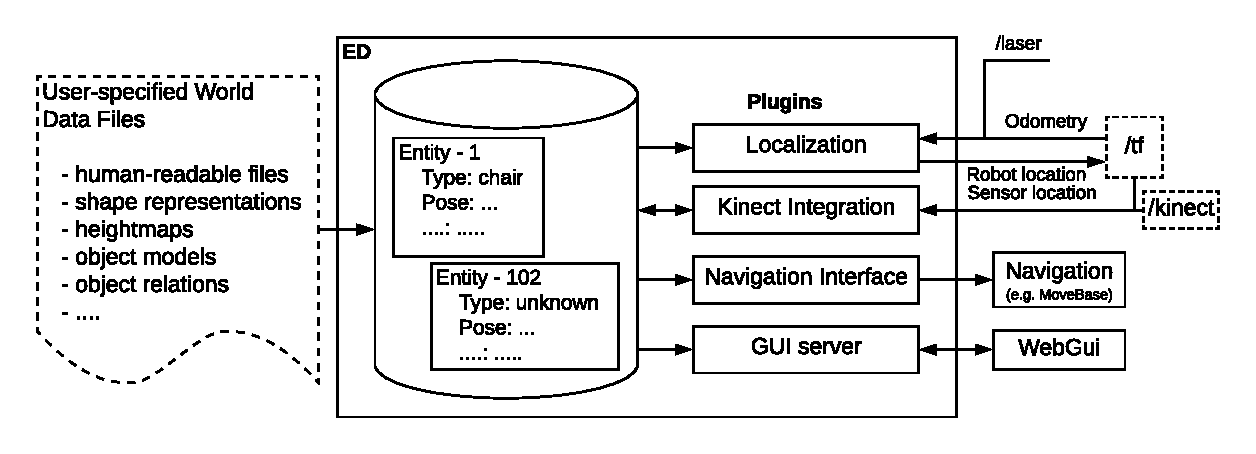
\includegraphics[width = 0.9\linewidth]{Figures/ed_overview}
    %\vspace{-1em}
	\caption{Schematic overview of TU/e Environment Descriptor.}
	\label{fig:ed}
    %\vspace{-0.5cm}
\end{figure}
ED is a single re-usable environment description that can be used for a multitude of desired functionalities instead of having different environment representations for localization, navigation, manipulation, interaction, etc.. An improvement in this single, central world model will reflect in the performances of the separate robot capabilities. It omits updating and synchronization of multiple world models. At the moment different \acrshort{ed} plugins exist that enable robots to localize themselves, update positions of known objects based on recent sensor data, segment and store newly encountered objects and visualize all this in RViz and through a web-based \acrshort{gui}, illustrated in Figure \ref{fig:gui_actions}.
\begin{figure}[h]
\centering
    %\vspace{-0.3cm}
	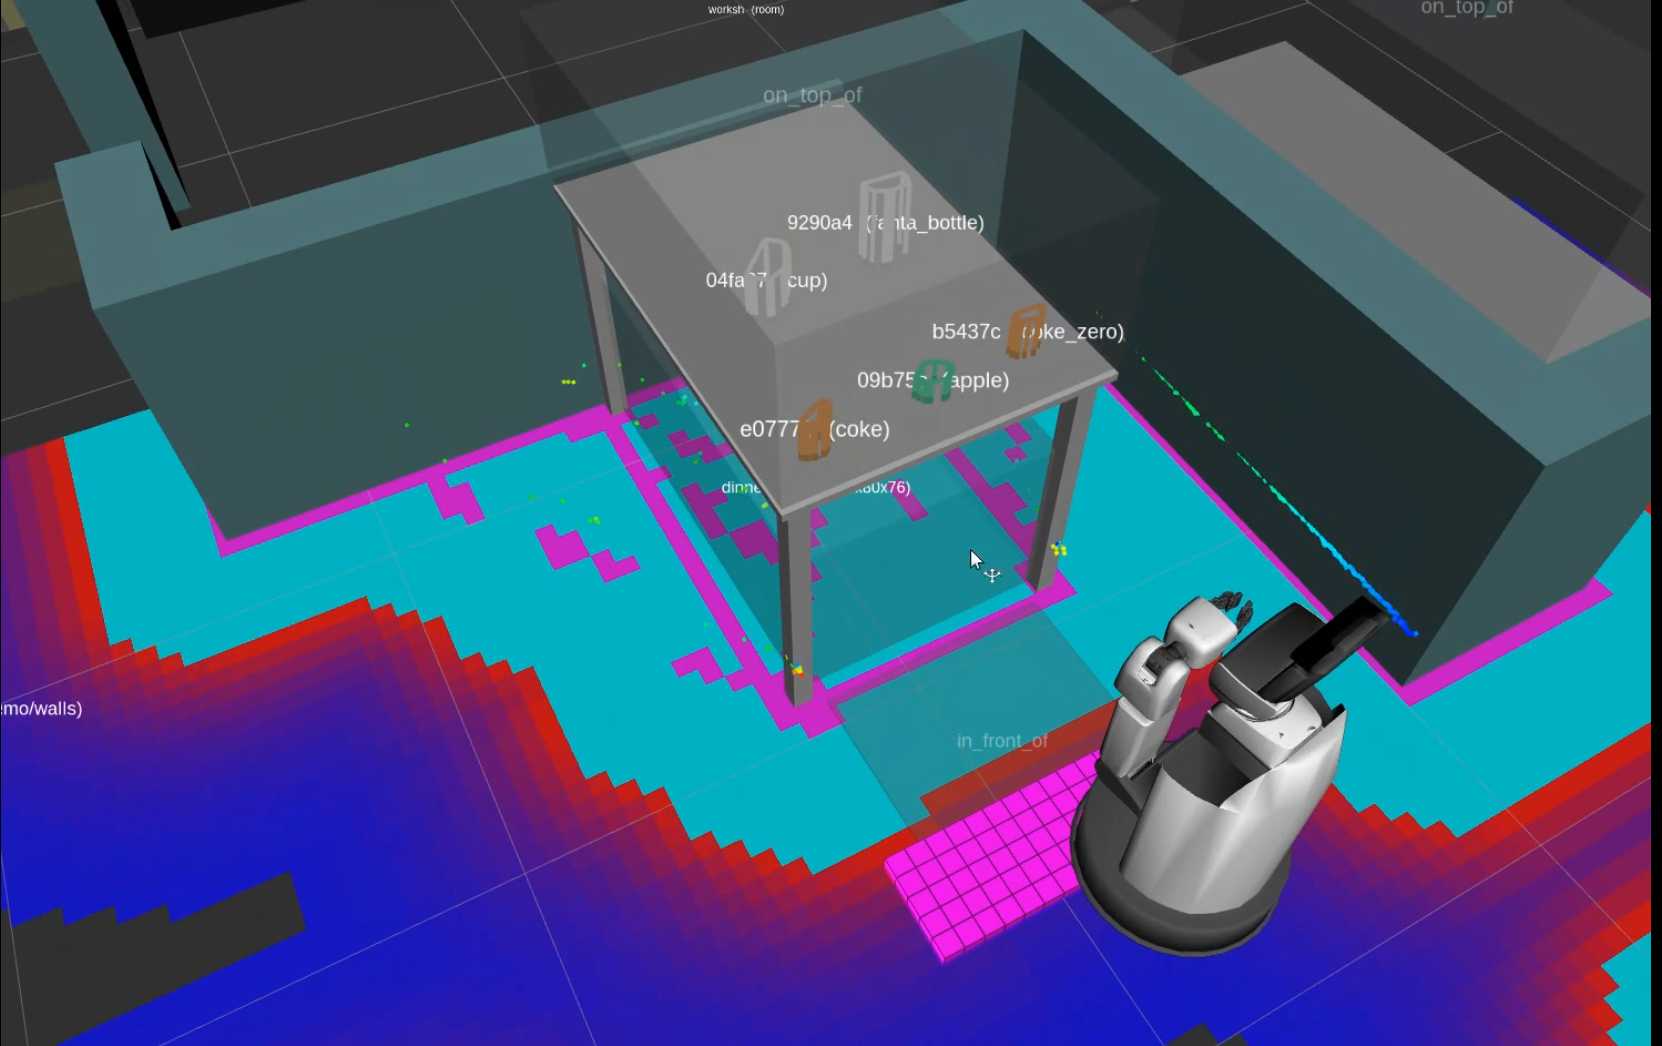
\includegraphics[width = 0.8\linewidth]{Figures/ed_segmentation_hsr}
    %\vspace{-0.5em}
	\caption{A view of the world model created with \acrshort{ed}. The figure shows the occupation grid as well as classified objects recognized on top of the cabinet.}
	\label{fig:ed_segmentation}
    %\vspace{-0.5cm}
\end{figure}
